\documentclass[10pt,twocolumn]{article}
\usepackage[a4paper,margin=1in]{geometry}
\usepackage{graphicx}
\usepackage{amsmath}
\usepackage{amsfonts}
\usepackage{hyperref}
\usepackage{lipsum} % For placeholder text

\title{DDM - lab 1 report}
\author{Arico Amaury\\Colot Emmeran}
\date{}
\begin{document}

\maketitle

\section{Objective}
The objective of this lab session is to establish a parametric model of a system. Once a model is obtained, the impact of some parameters will be studied such as the order of the model or the power of the noise. Finally, the optimal parameters will be chosen following some criterions (\textit{AIC} and \textit{validation dataset}).

\section{System under test}

The system under test is a Chebycheff passband filter of order 2. It's frequential and temporal characteristics are shown in figure \ref{fig:chebycheff}. 

\begin{figure}
    \centering
    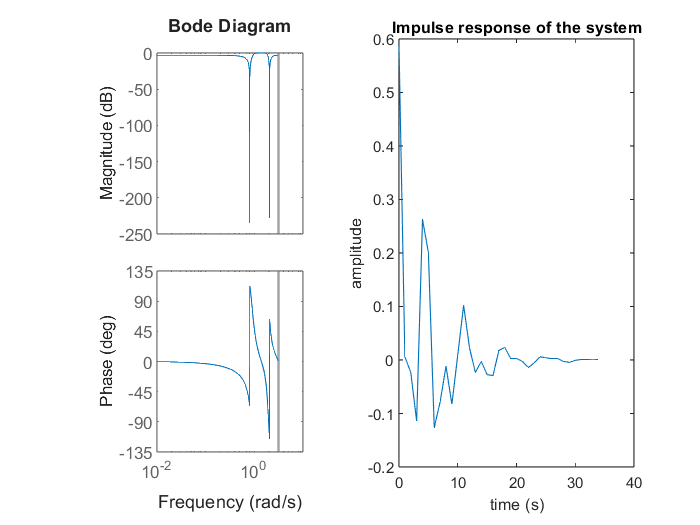
\includegraphics[width=0.5\textwidth]{pic/filterCaracteristics.png}
    \caption{Chebycheff filter of order 2}
    \label{fig:chebycheff}
\end{figure}

\section{Least Square Error Estimation}

The LLS estimation needs a regressor matrix $H_n$ that is built based on the signal $u[n]$ fed to the system. Because the chosen model is a FIR, the output depends only on the past values of the input:
\begin{equation}
    \label{eq:regressor}
    y[n] = \sum_{k=0}^{N_e-1} g_0[k] u[n-k] + v[n]
\end{equation}
Where $v[n]$ is the additive noise and $N_e$ the number of samples of the input signal. Transforming this equation into a matrix form gives:
\begin{equation}
    y[n] = H_n g_0 + v[n]
\end{equation}
The regressor matrix $H_n$ is built as follows to fit equation \ref{eq:regressor}:
\begin{equation}
    H_n = \begin{bmatrix}
        u[0] & 0 & \cdots & 0 \\
        u[1] & u[0] & \cdots & 0 \\
        \vdots & \vdots & \ddots & \vdots \\
        u[N_e-1] & u[N_e-2] & \cdots & u[N_e-n_p]
    \end{bmatrix}
\end{equation}
With $n_p$ the number of parameters of the model.

\section{Model order selection}

The curve of the cost function using the estimation dataset is strictly decreasing because by adding more parameters, one can only go towards a better fit. To determine the optimal number of parameters, we will use the \textit{AKAIKE Information Criterion} which corrects the LS cost function by factor penalizing the number of parameters:
\begin{equation}
    V_{AIC} = V_{LS} \left(1+\frac{2n_p}{N_e}\right)
\end{equation}
The other criterion is built using a validation dataset generated exactly like the estimation dataset. It means the values are independent from the dataset used for the parameters generation. This way, the noise that will be followed by an overfitting model will be detected. The curves are shown in figure \ref{fig:costFunction}. The optimal number of parameters are the one that minimizes the cost functions and it can be seen that the AIC and the validation dataset criterion give close values of $n_{p, \text{opt}}$.
\begin{figure}
    \centering
    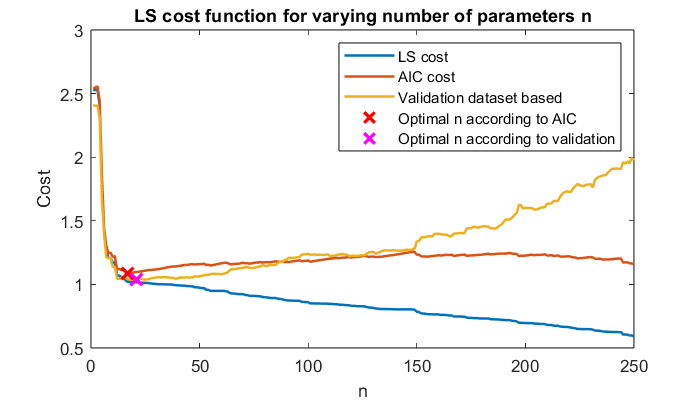
\includegraphics[width=0.5\textwidth]{pic/cost.png}
    \caption{Cost function for different model orders}
    \label{fig:costFunction}
\end{figure}

\section{Parameters effects}

\begin{itemize}
    \item \textbf{SNR}: Increasing the SNR will increase the value of the optimal number of parameters. It is easily understandable using the validation dataset criterion. A lower noise level means that the estimation and validation dataset are closer to each other, making the model fit better even with more parameters to the second dataset.
    \item \textbf{Bandwidth}: Reducing the bandwidth of the system under test will increase its complexity and therefore the number of parameters needed to fit the model. The same thing will happen if the order of the system is increased. 
    \item \textbf{Number of samples of the input signal}: The number of samples impacts mainly the AIC criterion as the cost is divided by $N_e$. The plots \ref{fig:lowSamples} and \ref{fig:highSamples} show that lowering the number of samples make the AIC criterion irrelevant whereas a higher number of samples makes the AIC cost curve and the validation dataset cost curve converge.
\end{itemize}

\begin{figure}
    \centering
    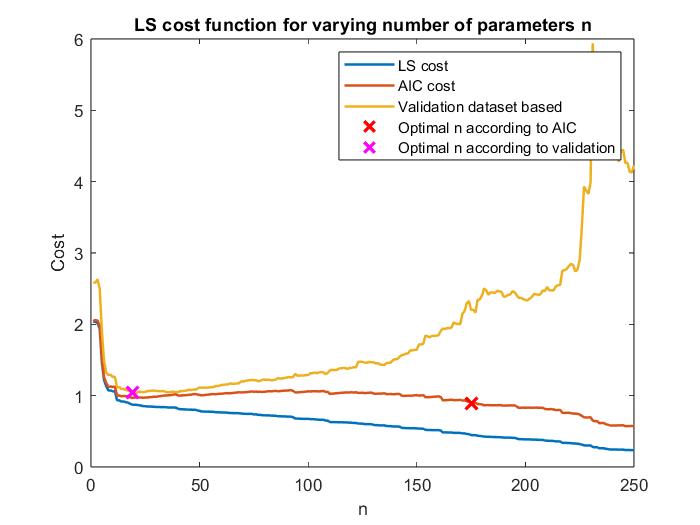
\includegraphics[width=0.5\textwidth]{pic/lowSamples.png}
    \caption{Cost function for different model orders with a low number of samples}
    \label{fig:lowSamples}
\end{figure}

\begin{figure}
    \centering
    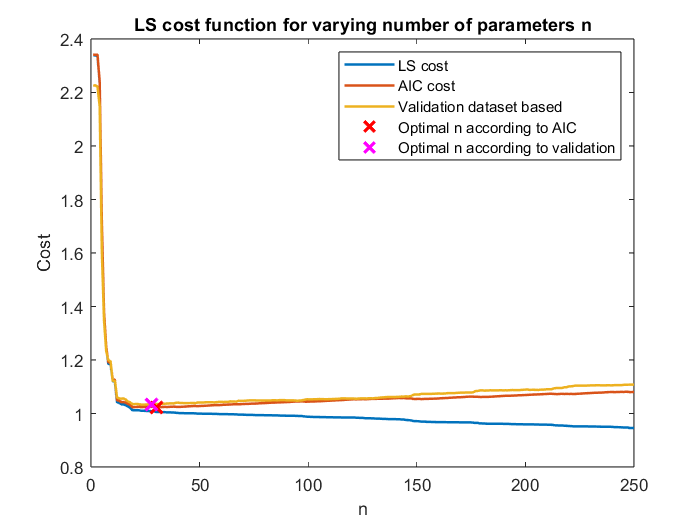
\includegraphics[width=0.5\textwidth]{pic/highSamples.png}
    \caption{Cost function for different model orders with a high number of samples}
    \label{fig:highSamples}
\end{figure}

\section{Model robustness}

As the input signal and the additive noise are random variables, the robustness of the model can be estimated by running the whole experiment several times and comparing the results. Figure \ref{fig:histogram} shows the distribution of the optimal number of estimated parameters for 100 runs. Even though it can vary, there is a clear tendency for $n_{\text{opti}}$ around 19. The averaged cost curves are also shown in figure \ref{fig:mean}. Their smoothness shows that the chosen criterions are a solid choice to estimate the optimal number of parameters.

\begin{figure}
    \centering
    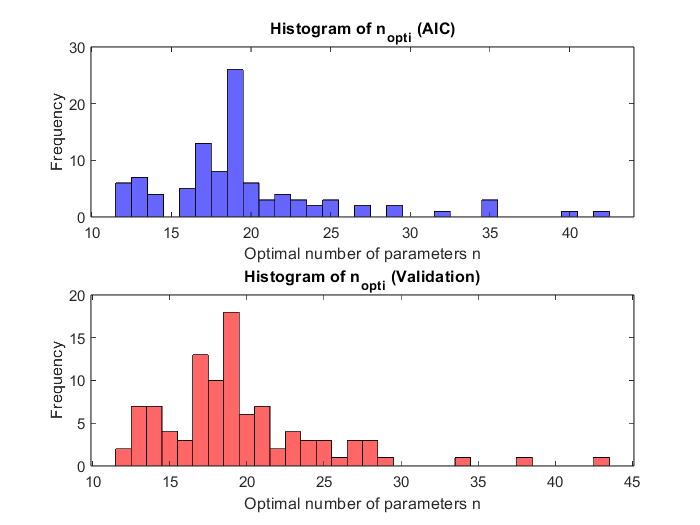
\includegraphics[width=0.5\textwidth]{pic/histogram.png}
    \caption{Histogram of the optimal number of parameters for 100 runs}
    \label{fig:histogram}
\end{figure}

\vspace{0cm} % Adjust the vertical spacing to fit the figure on the previous page
\begin{figure}[!ht]
    \centering
    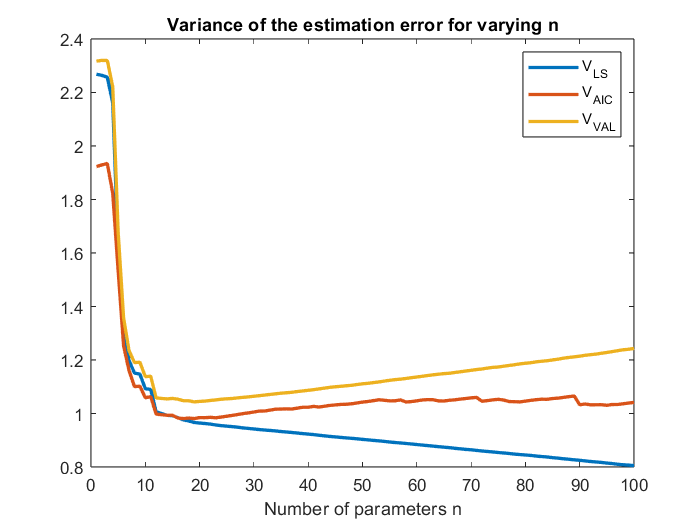
\includegraphics[width=0.4\textwidth]{pic/mean.png}
    \caption{Mean cost function for different model orders}
    \label{fig:mean}
\end{figure}

\end{document}